%\documentclass[slidestop,usepdftitle=false]{beamer}
\documentclass[blue]{beamer}
\usepackage[accumulated]{beamerseminar}
\usepackage{beamertexpower}
%\usepackage[brazil]{babel}
\usepackage[utf8]{inputenc}
\usepackage[portuges]{babel}
\usepackage{stmaryrd} %produto kulkarni-nomizu
\usepackage[normalem]{ulem}%para tachar/riscar o texto \sout{texto}
\usepackage{graphicx}
\usepackage{ragged2e}
\usepackage{graphicx,color}
\usepackage[all]{xy}
%\usepackage[latin1]{inputenc}
\usepackage{amssymb}
\usetheme{Darmstadt}\setbeamercolor{normal text}{}
\graphicspath{{figure/}}
%\usetheme{Hannover}\setbeamercolor{normal text}{bg=green!10}
\title[UFPA]{Equa��es diferenciais}
\author{Rafael Sergio Sampaio Emidio}
\institute
	{
		XXX Seminário de Iniciação Científica 2019 \\
		Bolsa PIBIC/PRODOUTOR \\
Instituto de Ci�ncias Exatas e Naturais\\
Orientador: Augusto C�sar dos Reis Costa}
\usetheme{Warsaw}
\newtheorem{proposition}{Proposição}
\newtheorem{cor}{Corolário}
\newtheorem{deff}{Definição}
\newtheorem{thm}{Teorema 1}
\newtheorem{lem}{Lema 1}
\newtheorem{lem2}{Lema 2}
\newtheorem{ex}{Example}
%\newtheorem{remark}{Remark}
\newtheorem{remark}{Observação}
\newtheorem{conjec}{Conjectura}
\newcommand{\Gij}[2]{\Gamma_{#1}^{#2}}
\begin{document}
\frame{\titlepage}
+++++++++


%$$$$$$$$$$$$$$$$$$$$$ PRIMEIRA LAMINA $$$$$$$$$$$$$$$$$$$$$$$$$$$$$$$$$$$
%$$$$$$$$$$$$$$$$$$$$$$$$$$$$$$$$$$$$$$$$$$$$$$$$$$$$$$$$$$$$$$$$$$$$$$$$$$
\begin{frame}
 \frametitle{Introdução}

%\hspace{0.5cm} O trabalho está composto como segue:\pause
\justify
 \hspace{0.2cm}O objetivo deste trabalho é mostrar que a esfera é uma superfície rígida através de relações entre propriedades locais e globais de curvas e superfícies da Geometria Diferencial. Iremos verificar que se uma superfície regular $S$ conexa e compacta possui curvatura gaussiana $K$ constante, então $S$ é uma esfera.\\
 \vspace{2cm}
 Palavras-chave: superfícies regulares, esfera, curvaturas.


\end{frame}
%
%
%
%%$$$$$$$$$$$$$$$$$$$$$$$$$$$$$$$$$$$$$$$$$$$$$$$$$$$$$$$$$$$$$$$$$$$$$$$$$
%%$$$$$$$$$$$$$$$$$$$$$$$$$$$$$$$$$$$$$$$$$$$$$$$$$$$$$$$$$$$$$$$$$$$$$$$$$
%
%
%
%
%
%%$$$$$$$$$$$$$$$$$$$$$ SEGUNDA LAMINA $$$$$$$$$$$$$$$$$$$$$$$$$$$$$$$$$$$
%%$$$$$$$$$$$$$$$$$$$$$$$$$$$$$$$$$$$$$$$$$$$$$$$$$$$$$$$$$$$$$$$$$$$$$$$$$
\begin{frame}
\frametitle{Superfície regular} 
\justify
\hspace{0.2cm}Uma superfície regular S é um subconjunto do espaço tal que para todo ponto p, existe uma aplicação $X: U \rightarrow V\cap S$, onde $U$ é um aberto em $R^2$, $V$ uma vizinhança de $p$ e $X$ satisfaz as seguintes condições:
\begin{enumerate}
	\item $X$ é diferenciável;
	\item $X$ é homeomorfismo;
	\item A diferencial $dX_q: R^2 \rightarrow R^3$ é injetiva.
\end{enumerate}
\end{frame}
%%$$$$$$$$$$$$$$$$$$$$$$$$$$$$$$$$$$$$$$$$$$$$$$$$$$$$$$$$$$$$$$$$$$$$$$$$$
%%$$$$$$$$$$$$$$$$$$$$$$$$$$$$$$$$$$$$$$$$$$$$$$$$$$$$$$$$$$$$$$$$$$$$$$$$$
\begin{frame}{Superfície regular}
\justify
\hspace{0.2cm}Neste caso, chamamos $X$ de um parametrização de $S$. Assim, dado $(u, v) \in U$ temos $X(u, v) = (x(u, v), y(u, v), z(u, v))$.
\begin{figure}[ht!]
	\centering
	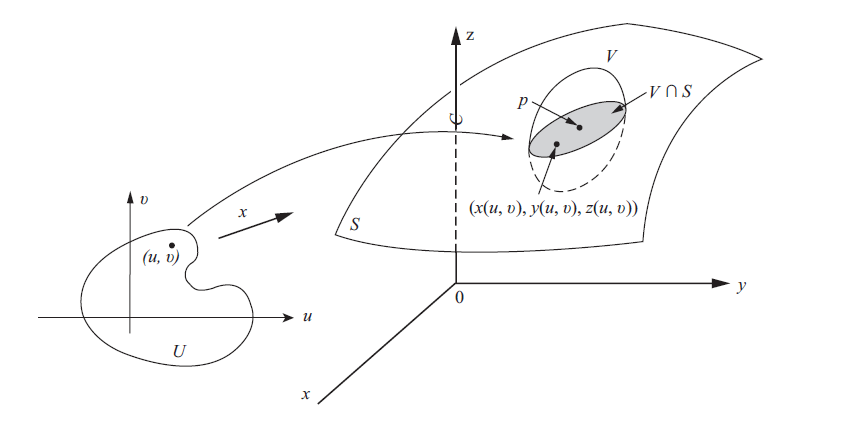
\includegraphics[width=12cm]{img1.png}
\end{figure}
\end{frame}
%
%
%
%%%%%%%%%%%%%%
\begin{frame}{Aplicação de Gauss} 
\justify
\hspace{0.2cm}Dada uma parametrização $X: U \subset R^2 \rightarrow S$ de uma superfície regular S em um ponto $p \in S$. Desde que \{$X_u$, $X_v$\} constitui uma base para $T_qS$, podemos definir para cada ponto $q \in X(U)$, um vetor normal unitário da seguinte maneira: 
$$
N(q)=\frac{X_u\wedge X_v}{|X_u\wedge X_v|}, \quad \quad q \in X(q) 
$$
\begin{figure}[ht!]
	\centering
	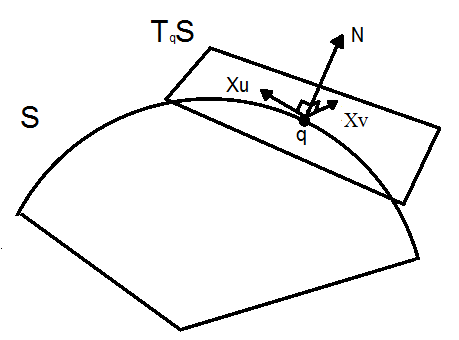
\includegraphics[width=5.8cm]{Img2.png}
	\end{figure}
\end{frame}

\begin{frame}
\justify
\hspace{0.2cm}Se a superfície $S$ possui uma orientação $N$, podemos garantir a existência da aplicação $N: S \rightarrow R^3$ que toma seus valores em uma esfera unitária
\begin{figure}[ht!]
	\centering
	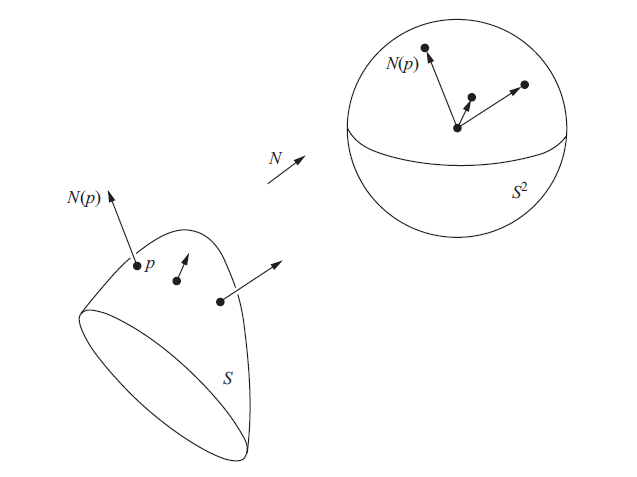
\includegraphics[width=5.5cm]{img4.png}
\end{figure}
\hspace{0.2cm}A aplicação $N: S \rightarrow S^2$ é chamada de aplicação normal de Gauss de $S$. Podemos verificar que a diferencial $dN_p: T_pS \rightarrow T_pS$ é uma aplicação linear auto-adjunta.
\end{frame}

\begin{frame}
\justify
\hspace{0.2cm}Portanto, para cada ponto $p \in S$ existe uma base ortonormal $\{e_1, e_2\}$ de $T_pS$, tal que
$$ dN_p(e_1) = -k_1e_1 $$
$$ dN_p(e_2) = -k_2e_2  $$
\hspace{0.2cm}Onde $k_1$ e $k_2$ são respectivamente, o máximo e o mínimo da segunda forma fundamental $\amalg_p (v) = - < dN_p(v), v>$, ou seja, são os valores extremos da curvatura normal em $p$, tal que $k_1 \geq k_2$. \\
Os autovalores $k_1$ e $k_2$ são chamados de curvaturas principais e os autovetores $e_1$ e $e_2$ são chamados de direções principais.

\end{frame}

\begin{frame}
\justify
\begin{itemize}
	\item \textbf{Curvatura gaussiana ($K$)}: É o determinante da diferencial $dN_p$ de $S$ em $p$
	\begin{equation}
	K=k_1k_2. \nonumber
	\end{equation}
	\item \textbf{Curvatura média ($H$)}: É o negativo do traço da diferencial $dN_p$ de $S$ em $p$:
	\begin{equation}
	H=\frac{1}{2}(k_1+k_2) \nonumber
	\end{equation}
\end{itemize}
\end{frame}

\begin{frame}
\justify
\hspace{0.2cm}Um ponto de uma superfície regular $S$ é chamado de:
\begin{enumerate}
	\item Elíptico se $K > 0$;
	\item Hiperbólico se $K < 0$;
	\item Parabólico se $K = 0$, com $dN_p \neq 0$;
	\item Planar se $dN_p = 0$. 
\end{enumerate}
Obs1: Se $k_1(p) = k_2(p)$ então dizemos que $p$ é um ponto umbílico de $S$. \\
Obs2: Se todos os pontos de uma superfície $S$ são umbílicos, então $S$ está contida em um plano ou em uma esfera.
\end{frame}

\begin{frame}{Aplicação de Gauss em coordenadas locais}
\justify
\hspace{0.2cm}Através do estudo da aplicação de Gauss em coordenadas locais, obtemos as seguintes equações para a curvatura Gaussiana $K$ e a curvatura média $H$:
$$
K=\frac{eg-f^2}{EG-F^2} \quad \quad \quad H=\frac{1}{2}\frac{eG-2fF+gE}{EG-F^2} 
$$
Onde:
\begin{itemize}
	\justifying
	\item $E$, $F$ e $G$ são os coeficientes da primeira forma fundamental $I_p(w)= <w,w> = |w|^2$;
	\item $e$, $f$ e $g$ são os coeficientes da segunda forma fundamental $\amalg(v) = - < dN_p(v), v>$.
\end{itemize}

\end{frame}

\begin{frame}{Equações de compatibilidade}
\justifying
\hspace{0.2cm}As equações de compatibalidade são dadas pelas fórmulas de Gauss e pelas equações de Mainardi-Codazzi. 
\begin{itemize}
	\justifying
	\item Os coeficientes $\Gij{ij}{k}$, $i$,$j$,$k = 1,2$ são chamados de símbolos de Christoffel, obtidos nas derivadas dos vetores $X_u$, $X_v$ e $N$.
\end{itemize}
\hspace{0.2cm}Feitas várias demonstrações, foram encontradas as quatro equações de compatibilidade:
\begin{equation}
(\Gij{12}{2})_u-(\Gij{11}{2})_v+\Gij{12}{1}\Gij{11}{2}+\Gij{12}{2}\Gij{12}{2}-\Gij{11}{2}\Gij{22}{2}-\Gij{11}{1}\Gij{12}{2}=-EK
\end{equation}
\begin{equation}
(\Gij{12}{1})_u-(\Gij{11}{1})_v+\Gij{12}{2}\Gij{12}{1}-\Gij{11}{2}\Gij{22}{1}=FK
\end{equation}
\begin{equation}
e_v-f_u=e\Gij{12}{1}+f(\Gij{12}{2}-\Gij{11}{1})-g\Gij{11}{2}
\end{equation}
\begin{equation}
f_v-g_u=e\Gij{22}{1}+f(\Gij{22}{2}-\Gij{12}{1})-g\Gij{12}{2}
\end{equation}

\end{frame}

\begin{frame}
\justify
Obs3: Equações de compatibilidade quando as curvas coordenadas são linhas de curvaturas ($F = f = 0$)
\begin{equation}
K=-\frac{1}{2\sqrt{EG}}\left\{\left(\frac{E_v}{\sqrt{EG}}\right)_v+\left(\frac{G_u}{\sqrt{EG}}\right)_u \right\} \tag{1} \label{gauss}
\end{equation}
\begin{equation}
e_v=\frac{E_v}{2}\left(\frac{e}{E}+\frac{g}{G}\right) \tag{3} \label{1}
\end{equation}
\begin{equation}
g_u=\frac{G_u}{2}\left(\frac{e}{E}+\frac{g}{G}\right) \tag{4} \label{2}
\end{equation}
\end{frame}

\begin{frame}{Rigidez da esfera}
\begin{thm}
	Seja $S$ uma superfície conexa e compacta com curvatura gaussiana $K$ constante. Então $S$ é uma esfera.
\end{thm}
\end{frame}

\begin{frame}
\justify
\hspace{0.2cm}Para provar o Teorema 1, serão necessários alguns resultados. Estes resultados serão demonstrados através de 2 lemas.
\begin{lem}
	\justify
	 \hspace{0.2cm}Seja $S$ uma superfície regular e $p \in S$ satisfazendo as seguintes condições:
	 \begin{enumerate}
	 	\item $K(p) > 0$; isto é, a curvatura gaussiana em $p$ é positiva.
	 	\item $p$ é ao mesmo tempo um ponto de máximo local da função $k_1$ e um ponto de mínimo local da função $k_2 (k_1 \geq k_2)$.
	 \end{enumerate}
     \hspace{0.2cm}Então $p$ é um ponto umbílico de $S$. 
\end{lem}
\end{frame}

\begin{frame}
\justifying
\underline{Demonstração}: Vamos supor que $p$ não é um ponto umbílico e obter uma contradição.\\
Se $p$ não é um ponto umbílico de $S$, podemos parametrizar uma vizinhança coordenada de $p$ por coordenadas $(u,v)$ tais que as curvas coordenas são linhas de curvaturas. Então vamos ter que $F = f = 0$. Logo as curvaturas principais $k_1$ e $k_2$ serão dadas por 
\begin{equation}
k_1=\frac{e}{E}, \quad \quad k_2=\frac{g}{G}. \label{3}
\end{equation}
\hspace{0.2cm}Nestas condições as equações (\ref{1}) e (\ref{2}) de Mainardi-Codazzi são escritas como
\begin{equation}
e_v=\frac{E_v}{2}(k_1+k_2) \label{4}
\end{equation}
\begin{equation}
g_u=\frac{G_u}{2}(k_1+k_2) \label{5}
\end{equation}

\end{frame}

\begin{frame}
\justifying
\hspace{0.2cm}Derivando a primeira equação de (\ref{3}) com relação a $v$ e usando (\ref{4}), obtemos
\begin{equation}
E(k_1)_v=\frac{E_v}{2}(-k_1+k_2) \label{6}
\end{equation}
\hspace{0.2cm}Analogamente, derivando a segunda equação de (\ref{3}) com relação $u$ e usando (\ref{5}), obtemos
\begin{equation}
E(k_2)_u=\frac{G_u}{2}(k_1-k_2) \label{7}
\end{equation}
\hspace{0.2cm}Por outro lado, quando $F = 0$, a formula de Gauss (\ref{gauss}) para $K$ se reduz
$$
K=-\frac{1}{2\sqrt{EG}}\left\{\left(\frac{E_v}{\sqrt{EG}}\right)_v+\left(\frac{G_u}{\sqrt{EG}}\right)_u \right\}
$$
\end{frame}

\begin{frame}
\justifying
\hspace{0.2cm}Logo,
\begin{equation}
-2KEG=E_{vv}+G_{uu}+ME_{v}+NG_u \label{8}
\end{equation}
\hspace{0.2cm}A partir de (\ref{6}) e (\ref{7}), obtemos expressões para Ev e Gu que depois de derivadas, introduzimos na equação (\ref{8}) obtendo
$$-2KEG=-\frac{2E}{k_1-k_2}(k_1)_{vv}+\frac{2G}{k_1-k_2}(k_2)_{uu}+\bar{M}(k_1)_v+\bar{N}(k_2)_u $$
Donde, 
\begin{equation}
-2(k_1-k_2)KEG=-2E(k_1)_{vv}+2G(k_2)_{uu}+\tilde{M}(k_1)_v+\tilde{N}(k_2)_u \label{9}
\end{equation}
\hspace{0.2cm}Como $k_1$ atinge um máximo local em $p$ e $k_2$ atinge um mínimo local em $p$, temos
$$(k_1)_v=0, \quad (k_2)_u=0, \quad (k_1)_{vv} \leq 0, \quad (k_2)_{uu} \geq 0 $$
em $p$. No entanto, isto implica que o segundo membro da equação (\ref{9})  é positivo ou nulo, o que é uma contradição, logo o ponto p é um ponto umbílico de $S$.
\end{frame}

\begin{frame}
\justifying
\begin{lem2}
	Uma superfície regular compacta $S \subset R^3$ tem pelo menos, um ponto elíptico.
\end{lem2}
\underline{Demonstração}: Como $S$ é compacta, $S$ é limitada. Portanto $S$ está contida em alguma esfera em $R^3$, consideremos uma esfera $\Sigma$. Através de sucessivas diminuições do raio da esfera $\Sigma$, obtemos um ponto onde a mesma irá tocar em $S$, chamaremos de ponto $p$. Portanto, $\Sigma$ e $S$ são tangentes em $p$. 
\end{frame}

\begin{frame}
\justifying
\hspace{0.2cm}Observando as sessões normais em $p$, notamos que qualquer curvatura normal de $S$ em $p$ é maior ou igual que a curvatura normal de $\Sigma$ em $p$. Logo concluímos que $K_{S(p)} \geq K_{\Sigma(p)} > 0$, portanto $p$ é um ponto elíptico desejado.
\begin{figure}[ht!]
	\centering
	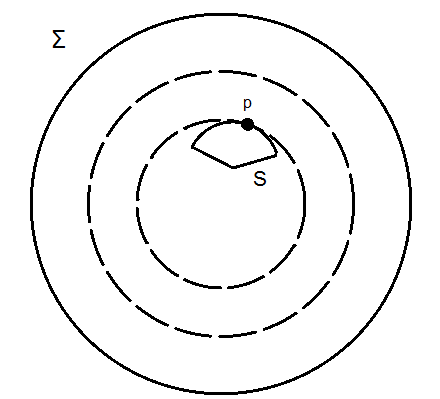
\includegraphics[width=5cm]{Img3.png}
\end{figure}
\end{frame}

\begin{frame}
\justifying
\textbf{Demonstração do teorema 1}: Como $S$ é compacta, ela possui um ponto elíptico pelo Lema 2. Como $K$ é constante, devemos ter $K > 0$ em $S$. Como $K = k_1k_2$ é uma constante positiva, $p$ é ao mesmo tempo o máximo local da função $k_1$ e o mínimo local da função $k_2$. Pelo lema 1 $p$ é um ponto umbílico de $S$, isto é, $k_1(p) = k_2(p)$. Agora seja um ponto $q \in S$, tal que $k_1(q) \geq k_2(q)$ temos
 \\ \vspace{0.3cm}
$$k_1(p) \geq k_1(q) \geq k_2(q) \geq k_2(p) = k_1(p). $$
\vspace{0.3cm} \\
\hspace{0.2cm}Portanto $k_1(q) = k_2(q)$ para todo $q \in S$. Podemos concluir de uma maneira definitiva que todos os pontos de S são umbílicos. Como $K > 0$, $S$ está contida em uma esfera $\Sigma$ pela observação 2. Por compacidade, $S$ é fechada em $\Sigma$, e como $S$ é uma superfície regular, $S$ é aberta em $\Sigma$. Como $\Sigma$ é conexa e $S$ é aberta e fechada em $\Sigma$, teremos que $S = \Sigma$. Portanto $S$ é uma esfera. 
\end{frame}

\begin{frame}{Bibliografia}
\justifying
DO CARMO, M. \textbf{Differential Geometry of curves and surfaces}. Pretince-Hall (1976)\\
TENEBLAT, K. \textbf{Introdução �  geometria diferencial}. Editora Blücher (2008)\\  
ARAÚJO, P. \textbf{Geometria Diferencial}. Coleção Matemática Universitária – IMPA (2004)
\end{frame}
%\begin{equation}
%
%\end{equation}

%\begin{frame}
%\centerslidesfalse \frametitle{Considerações iniciais}
%\pause
%Consideremos:
%\begin{itemize}
%	\item $(M^n, g)$ uma variedade Riemanniana conexa de dimensão $n\geq 3$;\pause
%	\item $\mathcal{M}$  o espaço das métricas Riemannianas suaves sobre $M$;\pause
%	\item $\mathcal{G}$ o grupo de difeomorfismos sobre $M$.\pause
%\end{itemize}
%\begin{block}{Definição:}
%Chamamos um funcional $\mathcal{F}: \mathcal{M} \rightarrow \mathbb{R}$ de Funcional Riemanniano, se ele é invariante pela ação do grupo $\mathcal{G}$, isto é, se $\mathcal{F}(\varphi^{\ast}g)= \mathcal{F}(g)$ para cada $\varphi\in \mathcal{G}$ e $g\in \mathcal{M}$.
%\end{block}
%\end{frame}
%
%
%%%%%%%%%%%%%%%%%%%%%%%%%%
%
%\begin{frame}{Gradiente de funcionais Riemannianos}\pause
%\begin{definition}
%	Um funcional Riemanniano $\mathcal{F}$ possui um gradiente em $g$, se existe $a\in \Gamma(S^{2}(T^{\ast}M))$ tal que para todo  $h\in \Gamma(S^{2}(T^{\ast}M))$,
%	$$\frac{\partial}{\partial t}\mathcal{F}(g(t))\Big|_{t=0} =\mathcal{F}'_{g}(h)=\langle a, h\rangle_{L^2}.$$
%\end{definition}\pause
%Neste caso, dizemos que $a$ é o gradiente de $\mathcal{F}$ e denotaremos por $a=\nabla \mathcal{F}$.
%\end{frame}
%
%\begin{frame}
%O \textbf{tensor curvatura de Riemann} é o $(1,3)-$tensor $ Rm:\mathfrak{X}(M)^3\rightarrow\mathfrak{X}(M)$ definido por
%\begin{eqnarray*}
%	Rm\,(X,Y)Z&=&\nabla_{X,Y}^{2}Z-\nabla_{Y,Z}^{2}Z\\
%	&=&\nabla_{X}\nabla_{Y}Z-\nabla_{Y}\nabla_{X}Z-\nabla_{[X,Y]}Z,
%\end{eqnarray*}
%para todo $X,Y,Z\in\mathfrak{X}(M).$\pause
%
%\begin{equation*}
%Rm\,(X,Y,Z,W)=-\langle Rm\,(X,Y)Z,W\rangle.
%\end{equation*}\pause
%
%Em coordenadas:
%\begin{eqnarray*}
%	Rm(\partial_{i}, \partial_{j})\partial_{k} &=&{R_{ijk}}^{l}\partial_{l}\\
%	Rm(\partial_{i}, \partial_{j}, \partial_{k}, \partial_{l}) &=&R_{ijkl}. 
%\end{eqnarray*}
%Assim,
%\begin{equation*}
%R_{ijkl} = - \langle Rm(\partial_{i}, \partial_{j})\partial_{k} , \partial_{l}\rangle = -\langle {R_{ijk}}^{m}\partial_{m}, \partial_{l}\rangle = -{R_{ijk}}^{m}g_{ml}, 
%\end{equation*}
%isto é, o índice superior desce na terceira posição. 
%\end{frame}
%
%\begin{frame}
%Dado um plano bidimensional $\Pi\subset T_{p}M$ e $X_{p}, Y_{p}\in T_{p}M$ vetores que geram $\Pi$, então
%\begin{equation}
%K(\Pi)=\frac{Rm(X, Y, X, Y)}{g(X, X)g(Y, Y)-g(X, Y)^{2}},
%\end{equation}
%não depende da base escolhida para $\Pi$, e é chamada {\bf curvatura seccional} do plano $\Pi$. \pause 
%
%Uma variedade Riemanniana completa e com curvatura seccional constante é dita uma {\bf forma espacial}.
%\end{frame}
%
%\begin{frame}
%O \textbf{tensor de Ricci} é definido como o $(0,2)-$ tensor
%\begin{equation*}
%{\rm Ric}(X,Y)= tr(U \rightarrow {\rm Rm}(U,X)Y).
%\end{equation*}
%Em coordenadas teremos:
%\begin{equation*}
%R_{ij} = {R_{lij}}^{l}= g^{lm}R_{limj}
%\end{equation*}
%e a \textbf{curvatura escalar} é
%\begin{equation*}
%R = g^{ij}R_{ij}.
%\end{equation*}
%\end{frame}
%
%
%%%%%%%%%%%%%%%%%%%%%%%%%%
%\begin{frame}{Motivação: Comparação de Volume}\pause 
%\begin{block}{(Bishop - Gromov, 1964)}
%	Seja $(M^n, g)$ uma variedade Riemanniana completa com $Ric \geq (n-1)kg$, $k$ constante, e $p\in M$ um ponto arbitrário. Então
%	$$Vol (B_{r}(p)) \leq Vol(B^{k}_{r}).$$ 
%\end{block}\pause
%
%Pergunta: \pause
%\begin{itemize}
%	\item \textcolor{blue}{controle na curvatura escalar}$ \Rightarrow $ \textcolor{red}{Comparação de volume ? 	}\pause
%\end{itemize}
%
%\begin{block}{Conjectura: (Schoen, 1989)}
%	Seja $(M^n, g)$ uma variedade hiperbólica fechada. Se $h$ é outra métrica sobre $M$ com $R_{h}\geq R_{g}$, então $Vol(h) \geq Vol(g)$.
%\end{block}
%
%\end{frame}
%
%\begin{frame}{(Miao -Tam, 2009)}\pause
%\begin{itemize}
%\item$(M^3, g)$ uma variedade Riemanniana com bordo $\partial M = \Sigma$.\pause
%\item $(\Sigma, \gamma)$ isometricamente mergulhada em $\mathbb{R}^{3}$ como uma hipersuperfície estritamente convexa $\Sigma_{0}$.\pause
%\item $g$ ponto crítico do funcional volume $V(.)$ sobre $\mathcal{M}_{\gamma}^{0} = \{g, R_{g} = 0 \; \mbox{e} \; g|_{\Sigma}= \gamma\}$.\pause
%\end{itemize}
%
%Então
%$$V_{g}\geq V_{0},$$
%com igualdade $\Leftrightarrow$ $(M, g)$ é isométrica �  bola Euclidiana padrão.
%
%\end{frame}
%
%
%
%
%%%%%%%%%%%%%%
%\begin{frame}{Motivação: Caracterização variacional}\pause
%Hilbert (1915): \pause
%\begin{block}{Funcional curvatura escalar total ou Funcional de Einstein-Hilbert}
%$$g \rightarrow \int_{M}R_{g} dV_{g},$$
%onde $R_{g}$ e $dV_{g}$ denotam, respectivamente, a curvatura escalar e a forma de volume de  $M^n$.
%\end{block}\pause
%
%\vspace{0.2cm}
%{\bf Relatividade Geral:} As equações de Einstein surgem como as equações de Euler-Lagrange desse funcional.
%\end{frame}
%
%
%
%
%
%
%
%
%%%%%%%%%%%%%%%%%%%%%%%
%
%\begin{frame}
%$$\mathcal{M}_{1}=\{g\in \mathcal{M} | Vol(g)=1\}$$\pause
%\begin{block}{(Hilbert, 1915)}
%Uma métrica $g\in\mathcal{M}_{1}$ é ponto crítico para o funcional de Einstein-Hilbert se, e somente se, $g$ é uma métrica de Einstein, isto é, $Ric_{g}=\frac{R_{g}}{n}g$.
%\end{block}\pause
%
%\vspace{0.2cm}
%Problema de Yamabe:\pause
%\begin{block}{(Schoen, 1984)}
%Dada uma variedade Riemanniana $(M,g)$, o funcional $$g \rightarrow Vol(g)^{-(n-2)/n}\int_{M}R_{g} dV_{g}$$ atinge um mínimo na classe conforme de $g$.
%\end{block}
%\end{frame}
%
%%%%%%%%%%%%%%%%%%%%%%%%
%%\begin{frame}
%%Relembremos que o tensor de Riemann admite a seguinte decomposição:\pause
%%\begin{eqnarray}
%%\label{weyl}
%%R_{ijkl}&=&W_{ijkl}+\frac{1}{n-2}\big(R_{ik}g_{jl}+R_{jl}g_{ik}-R_{il}g_{jk}-R_{jk}g_{il}\big) \nonumber\\
%%&&-\frac{R}{(n-1)(n-2)}\big(g_{jl}g_{ik}-g_{il}g_{jk}\big), 
%%\end{eqnarray}
%%de onde segue-se que\pause
%%\begin{eqnarray*}\label{Rie}
%%	\mathcal{R}(g)&=&\int_{M} |Rm_{g}|^2 dV_{g}\\
%%	& =& \int_{M} \left(|W_{g}|^2 + \dfrac{4}{n-2}|Ric_{g}|^2 - \dfrac{2}{(n-1)(n-2)}R_{g}^2\right)dV_{g}.
%%\end{eqnarray*}
%%\end{frame}
%
%%%%%%%%%%%%%%%%%%%%%
%
%
%
%
%%%%%%%%%%%%%%%%%%%%%%%%%%
%
%\begin{frame}
%Consideremos:\pause
%\begin{itemize}
%	\item $(M^n, g)$ uma variedade Riemanniana conexa, compacta e com bordo conexo suave $\Sigma$, $n\geq 3.$\pause
%	\item $\gamma$ uma métrica suave sobre $\Sigma$.\pause
%	\item $\mathcal{M}^{R}_{\gamma}=\{g\in \mathcal{M}; R_{g}=R \;\;\mbox{e}\;\; g|_{T\Sigma}=\gamma \}.$ \pause
%	\item O funcional volume $V : \mathcal{M}^{R}_{\gamma} \rightarrow \mathbb{R}$ dado por
%	$$V(g)=\int_{M}dV_{g}.$$
%\end{itemize}
%\end{frame}
%
%\begin{frame}{Caracterização variacional}\pause
%\begin{thm}[Miao e Tam, 2009]
%	Seja $g\in\mathcal{M}_\gamma^{R}$ tal que o primeiro autovalor de Dirichlet de $(n-1)\Delta_{g}+R$ é positivo.
%	Então $g$ é ponto crítico do funcional volume $V(\cdot)$ em $\mathcal{M}_\gamma^{R}$ se, e somente se, existe
%	uma função $f$ em $M$ satisfazendo o seguinte sistema de Equações Diferenciais Parciais
%	\begin{equation*}\label{teomotiveq1}
%	\left\{\begin{array}{rr}
%	-(\Delta_g f)g+\nabla_g^2f-fRic_g=g, &\mbox{ em } M\\
%	f=0, &\mbox{ sobre } \Sigma. \end{array} \right.
%	\end{equation*}
%\end{thm}\pause
%\begin{remark}
%	Se $(M,g)$ satisfaz $-(\Delta_g f)g+\nabla_g^2f-fRic_g=g$, então $R_{g}$ é constante.
%\end{remark}
%
%
%\end{frame}
%
%
%
%\begin{frame}
%
%\begin{deff}\
%Uma \textbf{métrica crítica de Miao-Tam}, ou simplesmente \textbf{métrica crítica}, é uma tripla $(M^{n},\,g,\,f)$, $n\geq 3$, onde $(M^n,\,g)$ é uma variedade
%Riemanniana compacta e conexa com bordo suave $\partial M=\Sigma$ e $f$ é uma função suave em $M$ tal que
%$f^{-1}(0)=\Sigma$ e satisfaz ao seguinte sistema de equações:
%\begin{equation*}
%\label{eqMiaoTam}-(\Delta_{g} f)g+\nabla_{g}^2f-fRic_{g}=g,
%\end{equation*}
%onde $\nabla_{g}^2 f$ denota o Hessiano de $f$. Tal função $f$ será chamada de função potencial.
%\end{deff}\pause
%
%\begin{block}{(Miao e Tam, 2009)}
%$g$ é ponto crítico de $V$ $\Leftrightarrow$ $g$ é uma métrica de Miao-Tam.
%\end{block}
%
%\end{frame}
%
%%%%%%%%%%%%%%%%%%%%%%
%\begin{frame}{Exemplos de métricas de Miao-Tam}\pause
%\begin{block}{Bola geodésica em $\mathbb{R}^{n}$}
%\begin{itemize}
%\item $(M^n, g)$ bola geodésica centrada na origem de raio $R_{0}$ em $\mathbb{R}^{n};$
%\item $f(x) = \frac{1}{2(n-1)}(R_{0}^{2}-|x|^{2}).$
%\end{itemize}
%\end{block}\pause
%\begin{block}{Bola geodésica em $\mathbb{H}^{n}$}
%\begin{itemize}
%\item $(M^n, g)$ bola geodésica centrada em $p\in \mathbb{H}^n$ de raio $R_{0};$
%\item $f(x) = \frac{1}{(n-1)}(1-\frac{\cosh r(x)}{\cosh R_{0}}).$
%\end{itemize}
%\end{block}\pause
%
%\begin{block}{Bola geodésica em $\mathbb{S}^{n}$}
%\begin{itemize}
%\item $(M^n, g)$ bola geodésica centrada em $p\in \mathbb{S}^n$ de raio $R_{0}<\frac{\pi}{2};$
%\item $f(x) = \frac{1}{(n-1)}(\frac{\cos r(x)}{\cos R_{0}}-1).$
%\end{itemize}
%\end{block}
%\end{frame}
%
%%%%%%%%%%%%%%%%%%%%%%%
%\begin{frame}{Alguns resultados existentes}\pause
%\begin{block}{(Miao e Tam, 2009)}
%Se $M$ é um domínio limitado com bordo suave em $\mathbb{R}^n,$ $\mathbb{H}^n$ ou $\mathbb{S}^n$ $($se
%$M^n\subset\mathbb{S}^n,$ suponha ainda que $V(M)<\frac{1}{2}V(\mathbb{S}^n)).$ Então a correspondente métrica
%nesse espaço é um ponto crítico do funcional volume $V(\cdot)$ em $\mathcal{M}_\gamma^{R}$ se, e somente se, $M$
%é uma bola geodésica.
%\end{block}\pause
%\begin{block}{Questão}
%As bolas geodésicas das formas espaciais simplesmente conexas $\mathbb{R}^n$, $\mathbb{S}^{n}$ e $\mathbb{H}^n$ são as únicas métricas críticas de Miao-Tam?\pause
%\\\textcolor{red}{Não!!!}
%\end{block}\pause
%\begin{block}{(Miao e Tam, 2011)}
%Construiram exemplos de métricas críticas conformemente planas que não são  métricas de Einstein.	
%\end{block}
%\end{frame}
%%%%%%%%%%%%%%%%%%%%%%%%%%%
%
%\begin{frame}
%
%\begin{block}{(Miao e Tam, 2011)}
%	Seja $(M^n,\,g,\,f)$ uma métrica crítica de Miao-Tam localmente conformemente plana, simplesmente conexa e com bordo $\Sigma$ isométrico �  esfera canônica $\mathbb{S}^{n-1}$. Então $(M^n,\,g)$ é isométrica a uma bola geodésica em $\mathbb{R}^n,$ $\mathbb{H}^n$ ou $\mathbb{S}^n.$
%\end{block}\pause 
%
%\begin{block}{(Miao e Tam, 2011)}
%Seja $(M^n,\,g,\,f)$ uma métrica crítica de Miao-Tam Einstein e bordo $\Sigma$ suave. Então $(M^n,\,g)$ é isométrica a uma bola geodésica em $\mathbb{R}^n,$ $\mathbb{H}^n$ ou $\mathbb{S}^n.$
%\end{block}
%
%\end{frame}
%
%
%\begin{frame}
%\begin{block}{Classificação de métricas críticas de Miao-Tam}
%	\begin{itemize}
%			\item (Barros-Diógenes-Ribeiro Jr, 2015)\\
%		\checkmark \textcolor{red}{n=4, simp. conexa, Bach-flat e $\Sigma \approx \mathbb{S}^{3}$}\pause
%	
%		\item (Kim-Shin, 2016)\\
%	\checkmark \textcolor{red}{n=4, simp. conexa, $divW = 0$ e $\Sigma \approx \mathbb{S}^{3}$ }\pause
%	
%		\item (Baltazar-Ribeiro Jr., 2017)\\
%		\checkmark \textcolor{red}{Ricci Paralelo}
%	
%		%\item (Baltazar-Ribeiro Jr., 2017)\\
%		%\checkmark \textcolor{red}{n=4, simp. conexa, $div^2W = 0$ e $\Sigma \approx \mathbb{S}^{3}$ }
%	\end{itemize}\pause
%	
%\end{block}
%\begin{block}{}
%	Em qualquer caso temos que $M^n$ é isométrica a uma bola geodésica em $\mathbb{R}^n,$ $\mathbb{H}^n$ ou $\mathbb{S}^n.$
%\end{block}
%\end{frame}
%
%
%
%
%
%%%%%%%%%%%%%%%%%%%
%
%%%%%%%%%%%%%%%%%%%%%%%%
%
%
%%%%%%%%%%%%%%%%%
%
%
%%%%%%%%%%%%%%%%%%%%%%%%%
%
%%%%%%%%%%%%%%%%%%%%%%%%%%%%%%
%\begin{frame}
%\begin{block}{(Batista-Diógenes-Raniere-Ribeiro Jr., 2016)}
%Seja $(M^3, g, f)$ uma métrica crítica de Miao-Tam, compacta, orientada, com bordo conexo $\Sigma$ e curvatura escalar não negativa. Então, $\Sigma$ é uma esfera bidimensional e 
%\begin{equation}\label{estMarcos}
%|\Sigma|\leq \frac{4\pi}{C(R)},
%\end{equation}
%onde $C(R)= \frac{R}{6} +\frac{1}{4|\nabla f|^2}$ é constante. Além disso, a igualdade em $(\ref{estMarcos})$ ocorre se, e somente se, $(M^3, g)$ é isométrica a bola geodésica em alguma forma espacial simplesmente conexa $\mathbb{R}^3$ ou $\mathbb{S}^3$.
%\end{block}\pause
%
%\begin{block}{Observação}
%Ainda em $2016$, E. Barbosa et al. mostraram que este resultado
% também é \textcolor{red}{válido} no caso de \textcolor{red}{curvatura escalar negativa}, supondo a curvatura média do bordo \textcolor{red}{$H>2$}.
% %\pause Além disso, provaram um resultado semelhante para dimensão \textcolor{red}{$n=5$} desde que o bordo \textcolor{red}{$\Sigma^{4}$ seja de Einstein}.
%\end{block}
%
%\end{frame}
%
%
%\begin{frame}{Estimativas e resultados de Rigidez}
%\begin{thm}[Barros, ---, 2017]
%	Seja $(M^n, g, f), \,n\geq 4,$ uma métrica crítica de Miao-Tam, compacta, orientada, com bordo conexo $\Sigma$ e curvatura escalar $R=n(n-1)\varepsilon $, onde $\varepsilon = -1, 0, 1$. Suponha que $\Sigma$ seja uma variedade de Einstein com curvatura escalar $R^{\Sigma}$ positiva. Se $\varepsilon = -1,$ assumimos ainda que a curvatura média de $\Sigma$ satisfaz $H> n-1$. Então temos
%	\begin{equation}\label{boundM}
%	|\Sigma|^{\frac{2}{n-1}} \leq \frac{Y(\mathbb{S}^{n-1}, [g_{can}])}{C(R)},
%	\end{equation}
%	onde $C(R)=\frac{n-2}{n}R+\frac{n-2}{n-1}H^{2}$ é uma constante positiva. Além disso, a igualdade ocorre em $(\ref{boundM})$ se, e somente se, $(M^n, g)$ é isométrica a uma bola geodésica em alguma das formas espaciais simplesmente conexas $\mathbb{S}^n$, $\mathbb{R}^{n}$ ou $\mathbb{H}^n$.
%\end{thm}
%\end{frame}
%
%
%
%%%%%%%%%%%%%%%%%%%%%%%%%%%%
%
%
%\begin{frame}{Considerações}\pause
%\begin{itemize}
%	\item $(M^n, g)$ variedade Riemanniana fechada de dimensão $n\geq 3;$\pause
%	\item $[g]$ a classe conforme de uma métrica $g\in \mathcal{M};$\pause
%	\item Constante de Yamabe: $$Y(M, [g]) = \inf_{\tilde{g}\in [g]} \frac{\int_{M} R_{\tilde{g}}dV_{\tilde{g}}} {(\int_{M}dV_{\tilde{g}})^{\frac{n-2}{n}}}.$$\pause
%	\item $Y(\mathbb{S}^{n}, [g_{can}]) = n(n-1)\omega_{n}^{2/n},$ onde $\omega_{n}$ denota o volume da esfera canônica unitária $\mathbb{S}^{n}$.
%\end{itemize}
%
%\end{frame}
%%%%%%%%%%%%%%%%%%%%%%%%%%%
%
%
%
%
%
%
%\begin{frame}{Fatos sobre métricas críticas de Miao-Tam}\pause
%	\begin{equation*}\label{Dirichlet}
%\begin{cases}
%-(\Delta_{g} f)g+\nabla_{g}^2f-fRic_{g}=g & \mbox{em}  \quad M\\
%f=0 & \mbox{sobre}  \quad \Sigma.
%\end{cases}
%\end{equation*}\pause
%
%\begin{itemize}
%	\item Curvatura escalar constante $R_{g}=n(n-1)\varepsilon$, onde $\varepsilon=-1,0,1$;\pause
%	\item $|\nabla f|$ é constante positiva sobre $\Sigma$;\pause
%	\item $\Sigma$ é uma hipersuperfície totalmente umbílica com curvatura média $H=\frac{1}{|\nabla f|}$;\pause
%	\item $2Ric(\nu, \nu) + R^{\Sigma} = R+ \frac{n-2}{n-1}H^2,$ onde $\nu =- \frac{\nabla f}{|\nabla f|}$ é o campo normal unitário exterior ao bordo $\Sigma$.
%\end{itemize}
%\end{frame}
%
%%%%%%%%%%%%%%%%%%%%%%%%%%%%%%%%%%
%
%\begin{frame}
%
%$$f\mathring{Ric}=\mathring{\nabla^{2}f}$$
%
%\begin{equation*}
%\label{divric}
%f|\mathring{Ric}|^2 = \langle \mathring{Ric}, \mathring{\nabla^2 f}\rangle = div(\mathring{Ric}(\nabla f)).
%\end{equation*}
%\begin{lemma}Seja $(M^n ,g, f)$ uma métrica crítica de Miao-Tam compacta, orientada, conexa e com bordo suave conexo $\Sigma$. Então,
%	\begin{equation*}
%	\int_{M}f|\mathring{Ric}|^2 dV_{g} = -H\int_{\Sigma}\mathring{Ric}(\nabla f, \nabla f) ds.
%	\end{equation*}
%\end{lemma}
%\end{frame}
%
%\begin{frame}
%\begin{proposition}\label{intRbound}
%	Seja $(M^n, g, f)$, $n\geq 3$, uma métrica crítica de Miao-Tam compacta, orientada, conexa, com bordo suave conexo $\Sigma$ e curvatura escalar $R= n(n-1)\varepsilon$, onde $\varepsilon = -1, 0, 1$. Então, a seguinte identidade ocorre
%	\begin{equation*}
%	\int_{\Sigma} R^{\Sigma} ds = 2H \int_{M} f|\mathring{Ric}|^2 dV_{g} + C(R)|\Sigma|,
%	\end{equation*}onde $C(R)$ é uma constante dada por $$C(R)=\frac{n-2}{n-1}(H^2 + (n-1)^2\varepsilon).$$
%	%	\begin{equation*}
%	% \int_{\Sigma} R^{\Sigma} ds = 2H \int_{M} f|\mathring{Ric}|^2 dV_{g} + \frac{n-2}{n-1}\big(H^2+\varepsilon (n-1)^2\big)|\Sigma|.
%	%\end{equation*}
%\end{proposition}
%\end{frame}
%
%
%
%%%%%%%%%%%%%%%%%%%%%%
%
%
%
%%%%%%%%%%%%%%%%%%%%%%%%%%%%%%%%
%
%\begin{frame}
%\begin{block}{(Ilias, 1983)}
%Seja $(M^n , g),\,n\ge 3,$ uma variedade Riemanniana compacta sem bordo. Suponha que $\mathcal{R}(M, g)\geq \mathcal{R}(\mathbb{S}^n , \frac{1}{\delta}g_{can})=(n-1)\delta>0$, então
%\begin{eqnarray*}
%\Big(\int_{M} |f|^{\frac{2n}{n-2}} dV_{g}\Big)^{\frac{n-2}{n}}&\leq &[K(n,2)]^2 \Big(\frac{\omega_{n}(\delta)}{|M|}\Big)^{\frac{2}{n}} \int_{M}|\nabla f|^2 dV_{g}\\
%& +& |M|^{-\frac{2}{n}}\int_{M} |f|^2 dV_{g},
%\end{eqnarray*}
%para toda $f\in H^{1,2}(M)$, onde $\omega_{n}(\delta)=\delta^{-\frac{n}{2}}\omega_{n}$.
%\end{block}
%
%\end{frame}
%
%%%%%%%%%%%%%%%%%%%%%%%%%5
%
%\begin{frame}
%\begin{block}{}
%	$$	\label{infric}\mathcal{R}(M, g) = \inf\{Ric(V, V) \;|\; V\in TM, |V|_{g}=1\};$$
%	$$K(n,2)= \sqrt{\frac{4}{n(n-2)\omega_{n}^{2/n}}}$$ é a melhor constante para desigualdades do tipo Sobolev:
%	\begin{equation}\label{sob1}
%	\Big(\int_{\Sigma} |\varphi|^{p} ds\Big)^{\frac{1}{p}}\leq A \Big(\int_{\Sigma}|\nabla \varphi|^{q} ds\Big)^{\frac{1}{q}} + B\Big(\int_{\Sigma} |\varphi|^{q} ds\Big)^{\frac{1}{q}},
%	\end{equation}onde $\frac{1}{p}=\frac{1}{q}-\frac{1}{n-1}$, $1\leq q <n-1$ e $q\in\mathbb{R}.$
%\end{block}
%\end{frame}
%
%
%\begin{frame}
%Aplicando �  variedade $\Sigma^{n-1}$ o teorema citado devido �  Ilias para  $\delta = \frac{R^{\Sigma}}{(n-1)(n-2)}>0$, obtemos
%\begin{eqnarray}
%\nonumber\Big(\int_{\Sigma} |\varphi|^{\frac{2(n-1)}{n-3}} ds\Big)^{\frac{n-3}{n-1}}&\leq& [K(n-1,2)]^2 \Big(\frac{\omega_{n-1}(\delta)}{|\Sigma|}\Big)^{\frac{2}{n-1}} \int_{\Sigma}|\nabla \varphi|^2 ds \\
%\nonumber &+& |\Sigma|^{-\frac{2}{n-1}}\int_{\Sigma} |\varphi|^2 ds,
%\end{eqnarray} para toda $\varphi\in H^{1,2}(\Sigma)$, onde $\omega_{n-1}(\delta)=\delta^{-\frac{n-1}{2}}\omega_{n-1}$, $\omega_{n-1} = |\mathbb{S}^{n-1}|$ e $K(n-1,2)$ é a melhor constante para desigualdades do tipo Sobolev.
%\end{frame}
%
%\begin{frame}
%\begin{eqnarray*}
%	\Big(\int_{\Sigma} |\varphi|^{\frac{2(n-1)}{n-3}} ds\Big)^{\frac{n-3}{2(n-1)}}&\leq &[K(n-1,2)] \Big(\frac{\omega_{n-1}(\delta)}{|\Sigma|}\Big)^{\frac{1}{n-1}}\Big( \int_{\Sigma}|\nabla \varphi|^2 ds\Big)^{\frac{1}{2}}\\
%	&+& |\Sigma|^{-\frac{1}{n-1}}\Big(\int_{\Sigma} |\varphi|^2 ds\Big)^{\frac{1}{2}}.
%\end{eqnarray*}\pause
%
%Com isto, temos
%	\begin{equation*}\label{ineqwsigma}
%(\omega_{n-1})^{\frac{2}{n-1}} \geq \delta |\Sigma|^{\frac{2}{n-1}}.
%\end{equation*}\pause 
%
%Substintuindo  $\delta = \frac{R^{\Sigma}}{(n-1)(n-2)}>0$, obtemos
%\begin{eqnarray}\label{ineqYam}
%Y(\mathbb{S}^{n-1}, [g_{can}]) \geq R^{\Sigma} |\Sigma|^{\frac{2}{n-1}}.
%\end{eqnarray}
%\end{frame}
%
%\begin{frame}{Prova}
%Integrando a equação anterior sobre $\Sigma$ e usando a Proposição acima, obtemos
%\begin{equation}\label{ineqSigY}
%|\Sigma|^{\frac{2}{n-1}} \leq \frac{Y(\mathbb{S}^{n-1}, [g_{can}])}{C(R)}.
%\end{equation} \pause
%Além disso, se ocorre a igualdade em \eqref{ineqSigY} devemos ter
%$$\int_{M} f|\mathring{Ric}|^2 dV_{g}=0.$$ Isto é, $(M^n,g)$ é uma variedade de Einstein.\pause  
%Logo, temos que $M^n$ é isométrica a uma bola geodésica em $\mathbb{R}^{n}$, $\mathbb{S}^{n}$ ou $\mathbb{H}^{n}$. \pause
%
%A recíproca?? \pause (Exercício)
%\end{frame}
%
%
%
%\begin{frame}
%\begin{cor}
%	Seja $(M^n, g, f), \,n\geq 4,$ uma métrica crítica de Miao-Tam, compacta, orientada, com bordo conexo $\Sigma$ isométrico �  esfera canônica $\mathbb{S}^{n-1}(r)$ de raio $r=\Big(\frac{(n-1)(n-2)}{C(R)}\Big)^{1/2}$, e curvatura escalar $R=n(n-1)\varepsilon $, onde $\varepsilon = -1, 0, 1$. Além disso, se $\varepsilon = -1,$ assumimos que a curvatura média de $\Sigma$ satisfaz $H> n-1$. Então $(M^n, g)$ é isométrica a uma bola geodésica em alguma das formas espaciais simplesmente conexas $\mathbb{S}^n$, $\mathbb{R}^{n}$ ou $\mathbb{H}^n$.
%\end{cor}\pause
%\begin{cor}
%	Com as mesmas condições do Teorema, porém $R\ge 0$, deduzimos
%	\begin{equation}\label{EstVolM}
%	\Big(\frac{nH}{n-1}\Big)^{\frac{2}{n-1}}|M|^{\frac{2}{n-1}}\leq \frac{Y(\mathbb{S}^{n-1}, [g_{can}])}{C(R)}.
%	\end{equation}
%	Ainda, a igualdade acontece em $(\ref{EstVolM})$ se, e somente se, $(M^n, g)$ é isométrica a uma bola geodésica no espaço euclidiano $\mathbb{R}^{n}$.
%\end{cor}
%\end{frame}

%%%%%%%%%%%%%%%%%%%%%%%%%%%%%%





%%%%%%%%%%%%%%%%%%%%%%%%%%%%%%%%%%%%%%%%%%%%%%%%%%%%%%%%%%%%%%%%%%%%%%%%%%%%%%%%%%%%%%%%%%%%%%%%%%%%%%%
%%%%%%%%%%%%%%%%%%%%%%%%%%%%%%%%%%%%%%%%%%%%%%%%%%%%%%%%%%%%%%%%%%%%%%%%%%%%%%%%%%%%%%%%%%%%%%%%%%%%%%%%%
%\begin{frame}
%\begin{thebibliography}{BB}
%\centerslidesfalse \frametitle{Refer\^encias}

%\bibitem{Baltazar} Baltazar, H.; Ribeiro Jr.: Critical metrics of the volume functional on manifolds with boundary. Proceedings of the American Mathematical Society, v. 145, p. 3513-3523, 2017.

%\bibitem{Barbosa} Barbosa, E.; Lima, L.; Freitas, A.: The generalized Pohozaev-Schoen identity and some geometric applications. arXiv:1607.03073v1 [math.DG], 2016.

%\bibitem{Batista} Batista, R.; Diógenes, R.; Raniere, M.; Ribeiro Jr.: Critical metrics of the volume functional on compact three-manifolds with smooth boundary. The Journal of Geometric Analysis, v. online, p. 1-18, 2016.

%\bibitem{Berger} Berger, M.: Quelques formules de variation pour une structure riemannienne. Annales Scientifiques de l'É.N.S., v. 3, n. 3, p. 285-294, 1970.




%\bibitem{ranieri} Batista, R.; Diógenes, R.; Ranieri, M; Ribeiro Jr., E.: Critical metric of the volume functional on compact three manifolds with smooth
%boundary. The Journal of Geometric Analysis, v. 27, p. 1530-1547, 2017.




%\end{thebibliography}{BB}
%\end{frame}

%%%%%%%%%%%%%%%%%%%%%%%%%%%%%%%%

%\begin{thebibliography}{BB}

%\bibitem{Besse} Besse, A.: Einstein Manifolds. New York: Springer-Verlag, 1987.

%\bibitem{Bou} Boucher, W.; Gibbons, G.; Horowitz, G.: Uniqueness theorem for anti-de Sitter spacetime. Physical Review D, v. 30, p. 2447-2451, 1984.


%\bibitem{Catino} Catino, G.: Some rigidity results on critical metrics for quadratic functionals. Calculus of Variations, v. 54, p. 2921-2937, 2015.

%\bibitem{Corvino} Corvino, J.: Scalar curvature deformation and a gluing construction for the Einstein constraint equations. Communications in Mathematical Physics, v. 214, n. 1, p. 137-189, 2000.

%\bibitem{Gur} Gursky, M.; Viaclovsky, J.: A new variational characterization of three-dimensional space forms. Inventiones Mathematicae, v. 145, p. 251-278, 2001.

%\bibitem{Hilbert} Hilbert, D.: Die Grundlagen der Physik. Annales Scientifiques de l'É.N.S., v. 4, p. 461-472, 1915.

%\bibitem{Hu} Hu, Z.; Li, H.: A new variational characterization of n-dimensional space forms. Transactions of the American Mathematical Society, v. 356, n. 8, p. 3005-3023, 2003.

%\bibitem{Huang} Huang, G.: Some rigidity characterizations on critical metrics for quadratic curvature functionals. arXiv: 1707.04806v1 [math.DG], 2017.

%\bibitem{Ilias} Ilias, S.: Constantes explicites pour les inégalités de Sobolev sur les variétés riemanniennes compactes. Annales de l'institut Fourier, v. 33, n. 2, p. 151-165, 1983.

%\bibitem{Kob} Kobayashi, O.: A differential equation arising from scalar curvature function. Journal of the Mathematical Society of Japan, v. 34, n. 4, p. 665-675, 1982.

%\bibitem{Lafon} Lafontaine, J.: Sur la géométrie d'une généralisation de l'équation différentielle d'Obata. Journal de Mathématiques Pures et Appliquées, v. 62, n. 1, p. 63-72, 1983.

%\bibitem{miaotam} Miao, P.; Tam, L.-F.: On the volume functional of compact manifolds with boundary with constant scalar curvature. Calculus of Variations and
%Partial Differential Equations, v. 36, n. 2, p. 141-171, 2009.

%\bibitem{miaotrans} Miao, P.; Tam, L.-F. Einstein and conformally at critical metrics of the volume functional. Transactions of the American Mathematical
%Society, v. 363, n. 6, p. 2907-2937, 2011.

%\bibitem{Qing} Qing, J.; Yuan, W.: A note on static spaces and related problems. J. Geom. and Phys., v. 74, p. 18-27, 2013.

%\bibitem{Schoen} Schoen, R.: Conformal deformation of a Riemannian metric to constant scalar curvature. Journal of Differential Geometry, v. 20, n. 2, p. 479-495, 1984.

%\bibitem{Shen} Shen, Y.: A note on Fischer-Marsden's conjecture. Proceedings of the American Mathematical Society, v. 125, n. 3, p. 901-905, 1997.

%\bibitem{Tanno} Tanno, S.: Deformations of Riemannian metrics on 3-dimensional manifolds. Tôhoku Mathematical Journal , v. 27, n. 3, p. 437-444, 1975.



%\bibitem{AA} Anderson, M.: Scalar curvature, metric degenerations and the static vacuum Einstein equations on 3-manifolds. Geom. and Funct. Anal., v. 9, p. 855-967, 1999.

%\bibitem{AC} Bunting, G.L., Masood-ul-Alam, A.K.M.: Non-existence of multiple black holes in asymptotically Euclidean static vacuum space-times.  Glasgow Math. J., v. 19, p. 147-154, 1987.

%\bibitem{CHE} Israel, W.: Event horizons in static vacuum space-time. Phys. Rev., v. 164, p. 1776-1779, 1967.
%p. 139-148, 2014.

%\bibitem{HE} Hwang, S., Chang, J., Yun, G.: Nonexistence of multiple black holes in static space-times and weakly harmonic curvature. Gen. Relativ. Gravit., v. 48, p. 120, 2016.

%%%%%%%%%%%%%%%%%%%%%%%%%%%%%%%%%%%%%%%%%%%%%%%%%
%\end{thebibliography}
\begin{frame}
\resizebox{!}{1cm}{\hspace{.4cm}Obrigado pela} \\
\resizebox{!}{1cm}{\hspace{.8cm}atenção!}
%\begin{figure}[ht]
%	\centering
%  \includegraphics[width=8cm, height=5cm]{RORAIMA.png}
%	%\caption{Jean-Pierre Bourguignon(francês)}
%	\label{fig1}
%\end{figure}\pause
\end{frame}
\end{document}





